\documentclass{article}
\usepackage[paperwidth=27cm,paperheight=15cm,margin=5mm]{geometry}
\usepackage{tikz}
\usepackage{amsmath}
\usetikzlibrary{arrows.meta,positioning,calc,fit,backgrounds,shapes.geometric}
\pagestyle{empty}
\definecolor{cdata}{RGB}{60,90,150}
\definecolor{cproc}{RGB}{40,140,95}
\definecolor{cefn}{RGB}{150,60,150}
\definecolor{cout}{RGB}{200,80,40}
\definecolor{cphi}{RGB}{235,170,40}
\begin{document}
\noindent
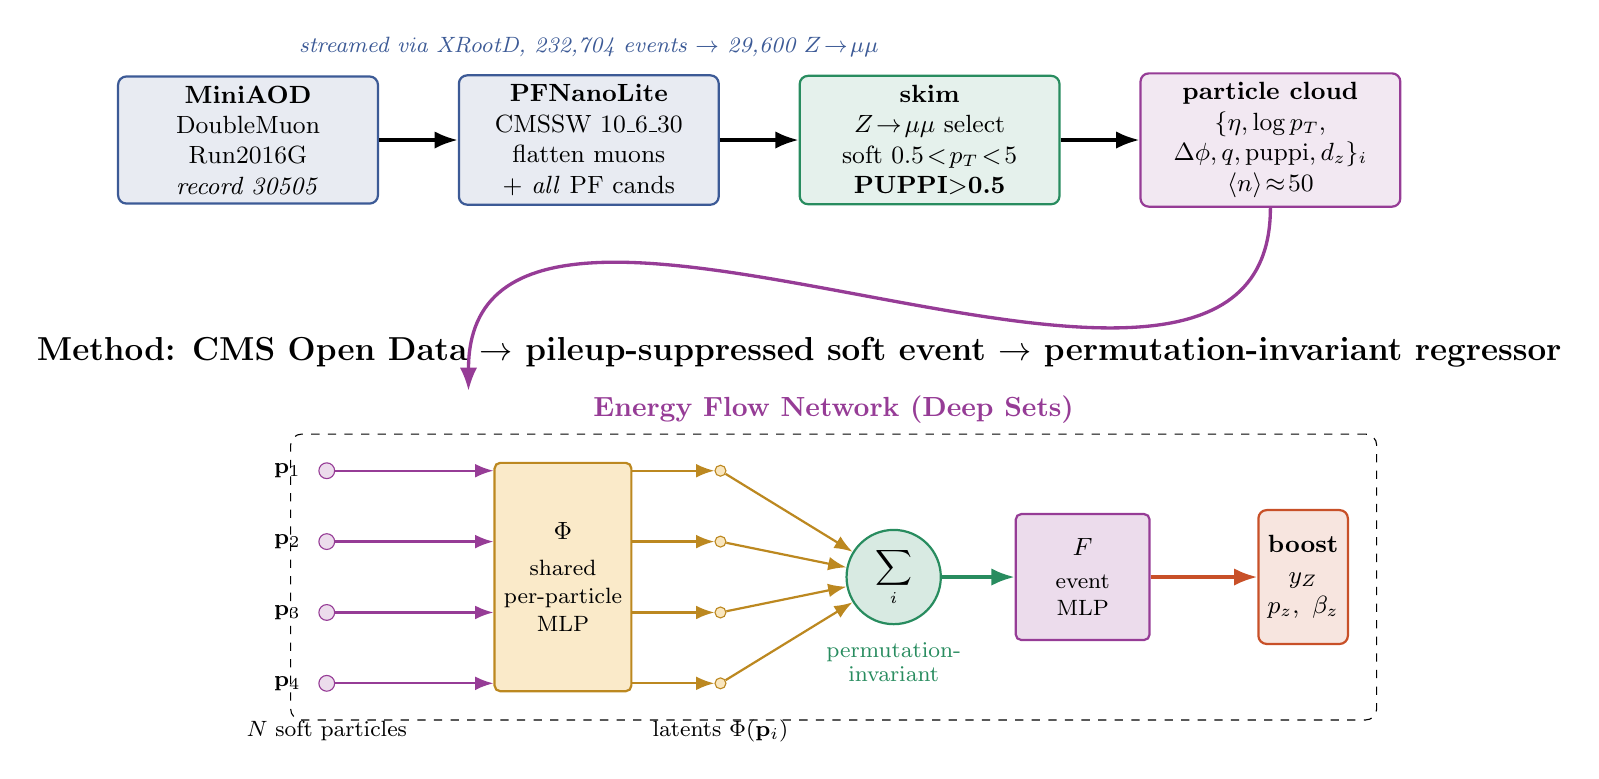
\begin{tikzpicture}[>=Latex,font=\sffamily,
  stage/.style={draw,thick,rounded corners=3pt,align=center,minimum height=1.5cm,minimum width=3.3cm,fill=#1!12,draw=#1},
  every node/.style={font=\small}]

% ===== top pipeline =====
\node[stage=cdata] (mini) {\textbf{MiniAOD}\\ DoubleMuon\\ Run2016G\\ \textit{record 30505}};
\node[stage=cdata,right=1.0cm of mini] (pf) {\textbf{PFNanoLite}\\ CMSSW $10\_6\_30$\\ flatten muons\\ $+$ \emph{all} PF cands};
\node[stage=cproc,right=1.0cm of pf] (skim) {\textbf{skim}\\ $Z\!\to\!\mu\mu$ select\\ soft $0.5\!<\!p_T\!<\!5$\\ \textbf{PUPPI$>$0.5}};
\node[stage=cefn,right=1.0cm of skim] (cloud) {\textbf{particle cloud}\\ $\{\eta,\log p_T,$\\ $\Delta\phi,q,\mathrm{puppi},d_z\}_i$\\ $\langle n\rangle\!\approx\!50$};
\foreach \a/\b in {mini/pf,pf/skim,skim/cloud}{\draw[->,very thick] (\a) -- (\b);}
\node[above=1mm of pf,font=\footnotesize\itshape,cdata]{streamed via XRootD, 232{,}704 events $\to$ 29{,}600 $Z\!\to\!\mu\mu$};

% ===== EFN block (below) =====
% particles
\foreach \i/\y in {1/-4.2,2/-5.1,3/-6.0,4/-6.9}{
  \node[draw,circle,inner sep=1.6pt,fill=cefn!18,draw=cefn] (p\i) at (1.0,\y) {$\,$};
  \node[left=1mm of p\i,font=\footnotesize] {$\mathbf{p}_\i$};
}
\node[font=\footnotesize] at (1.0,-7.5) {$N$ soft particles};
% shared Phi
\node[draw,thick,rounded corners=2pt,fill=cphi!25,draw=cphi!80!black,minimum height=2.9cm,minimum width=1.7cm,align=center] (phi) at (4.0,-5.55) {$\Phi$\\[2pt]\footnotesize shared\\[-1pt]\footnotesize per-particle\\[-1pt]\footnotesize MLP};
\foreach \i in {1,2,3,4}{\draw[->,thick,cefn] (p\i) -- (phi.west|-p\i);}
% latents
\foreach \i/\y in {1/-4.2,2/-5.1,3/-6.0,4/-6.9}{
  \node[draw,circle,inner sep=1.4pt,fill=cphi!30,draw=cphi!80!black] (z\i) at (6.0,\y) {};
  \draw[->,thick,cphi!80!black] (phi.east|-z\i) -- (z\i);}
\node[font=\footnotesize] at (6.0,-7.5){latents $\Phi(\mathbf{p}_i)$};
% sum pool
\node[draw,circle,thick,minimum size=1.1cm,fill=cproc!18,draw=cproc] (sum) at (8.2,-5.55) {$\displaystyle\sum_i$};
\foreach \i in {1,2,3,4}{\draw[->,thick,cphi!80!black] (z\i) -- (sum);}
\node[below=1mm of sum,font=\footnotesize,cproc,align=center]{permutation-\\[-1pt]invariant};
% F MLP
\node[draw,thick,rounded corners=2pt,fill=cefn!18,draw=cefn,minimum height=1.6cm,minimum width=1.7cm,align=center] (F) at (10.6,-5.55) {$F$\\[1pt]\footnotesize event\\[-1pt]\footnotesize MLP};
\draw[->,very thick,cproc] (sum) -- (F);
% outputs
\node[draw,thick,rounded corners=3pt,fill=cout!15,draw=cout,align=center,minimum height=1.7cm] (out) at (13.4,-5.55) {\textbf{boost}\\ $y_Z$\\ $p_z,\ \beta_z$};
\draw[->,very thick,cout] (F) -- (out);

% box around EFN
\begin{scope}[on background layer]
\node[draw,dashed,rounded corners=4pt,fit=(p1)(phi)(z1)(sum)(F)(out),inner sep=10pt,label={[font=\bfseries,cefn]above:Energy Flow Network (Deep Sets)}] {};
\end{scope}

% connect cloud -> EFN
\draw[->,very thick,cefn] (cloud.south) to[out=-90,in=90] ($(phi.north)+(-1.2,0.9)$);

% headline
\node[font=\bfseries\large,align=center] at (7.0,-2.7)
  {Method: CMS Open Data $\to$ pileup-suppressed soft event $\to$ permutation-invariant regressor};
\end{tikzpicture}
\end{document}
